\section{Introduktion til mapping}
Behovet for at fremskaffe et kort over en robots omgivelser vil i den ene eller anden forstand altid være påkrævet før robotten er i stand til at interagere med det miljø den er placeret i.
Det kan f.eks. være et stort udendørs areal man ønsker at bygge et kort over, eller f.eks. robottens eget syn på den verden hvori den bevæger sig.

Der findes flere afprøvede metoder indenfor robotik der gør det muligt for en robot at navigere og bygge kort over dens umiddelbare nærmeste omgivelser.
Dette afsnit vil fokusere på to af disse, navnligt \textit{Occupancy Grid} og \textit{Particle Filters}, og give en overordnet beskrivelse der skal danne grundlag for valget af metode for den fortløbende udvikling af projektet.
Afslutningsvis vil de to metoder blive sammenlignet for at belyse eventuelle fordele og ulemper ved begge.

\section{Notation}
Da det er ønskværdigt at kunne give en præcis beskrivelse af robottens position, positur og hvordan den bevæger sig, vil dette afsnit kort introducere den nødvendige notation, som foreslået af \citet{probabilisticRobotics}.


\section{Occupancy Grids}
Disse er en familie af algoritmer som gør det muligt at generere konsistente kort ud fra målinger med usikkerhed og støj (upræcise sensor målinger).
Da et \textit{occupancy grid map} går ud fra at robottens positur er kendt, kan disse med fordel overvejes til projektet, da dens lokation bestemmes eksternt via en Microsoft Kinect. \cite{probabilisticRobotics}

\subsection{Overblik}
Den overordnede idé bag et occupancy grid er at lave en ensartet inddeling af sit kort, hvor hver enkelt celle er repræsenteret af en binær tilfældig variabel der fortæller om den pågældende celle er 'optaget' eller ej, hvor optaget betegnes som sandsynligheden $\mathcal{P}(occupied) = 1$.
Til at begynde med initialiseres hver enkelt celle med værdien $\mathcal{P}(occupied) = 0,5$ som en indikation på den aktuelle tilstand endnu ikke er kendt.
En 'ledig' celle har således værdien $\mathcal{P}(occupied) = 0$.

En simpel illustration af et occupancy grid map for det kørselsmiljø der er opstillet for vores robot kan ses på \cref{map:occupancy_grid}.

\begin{figure}
\centering
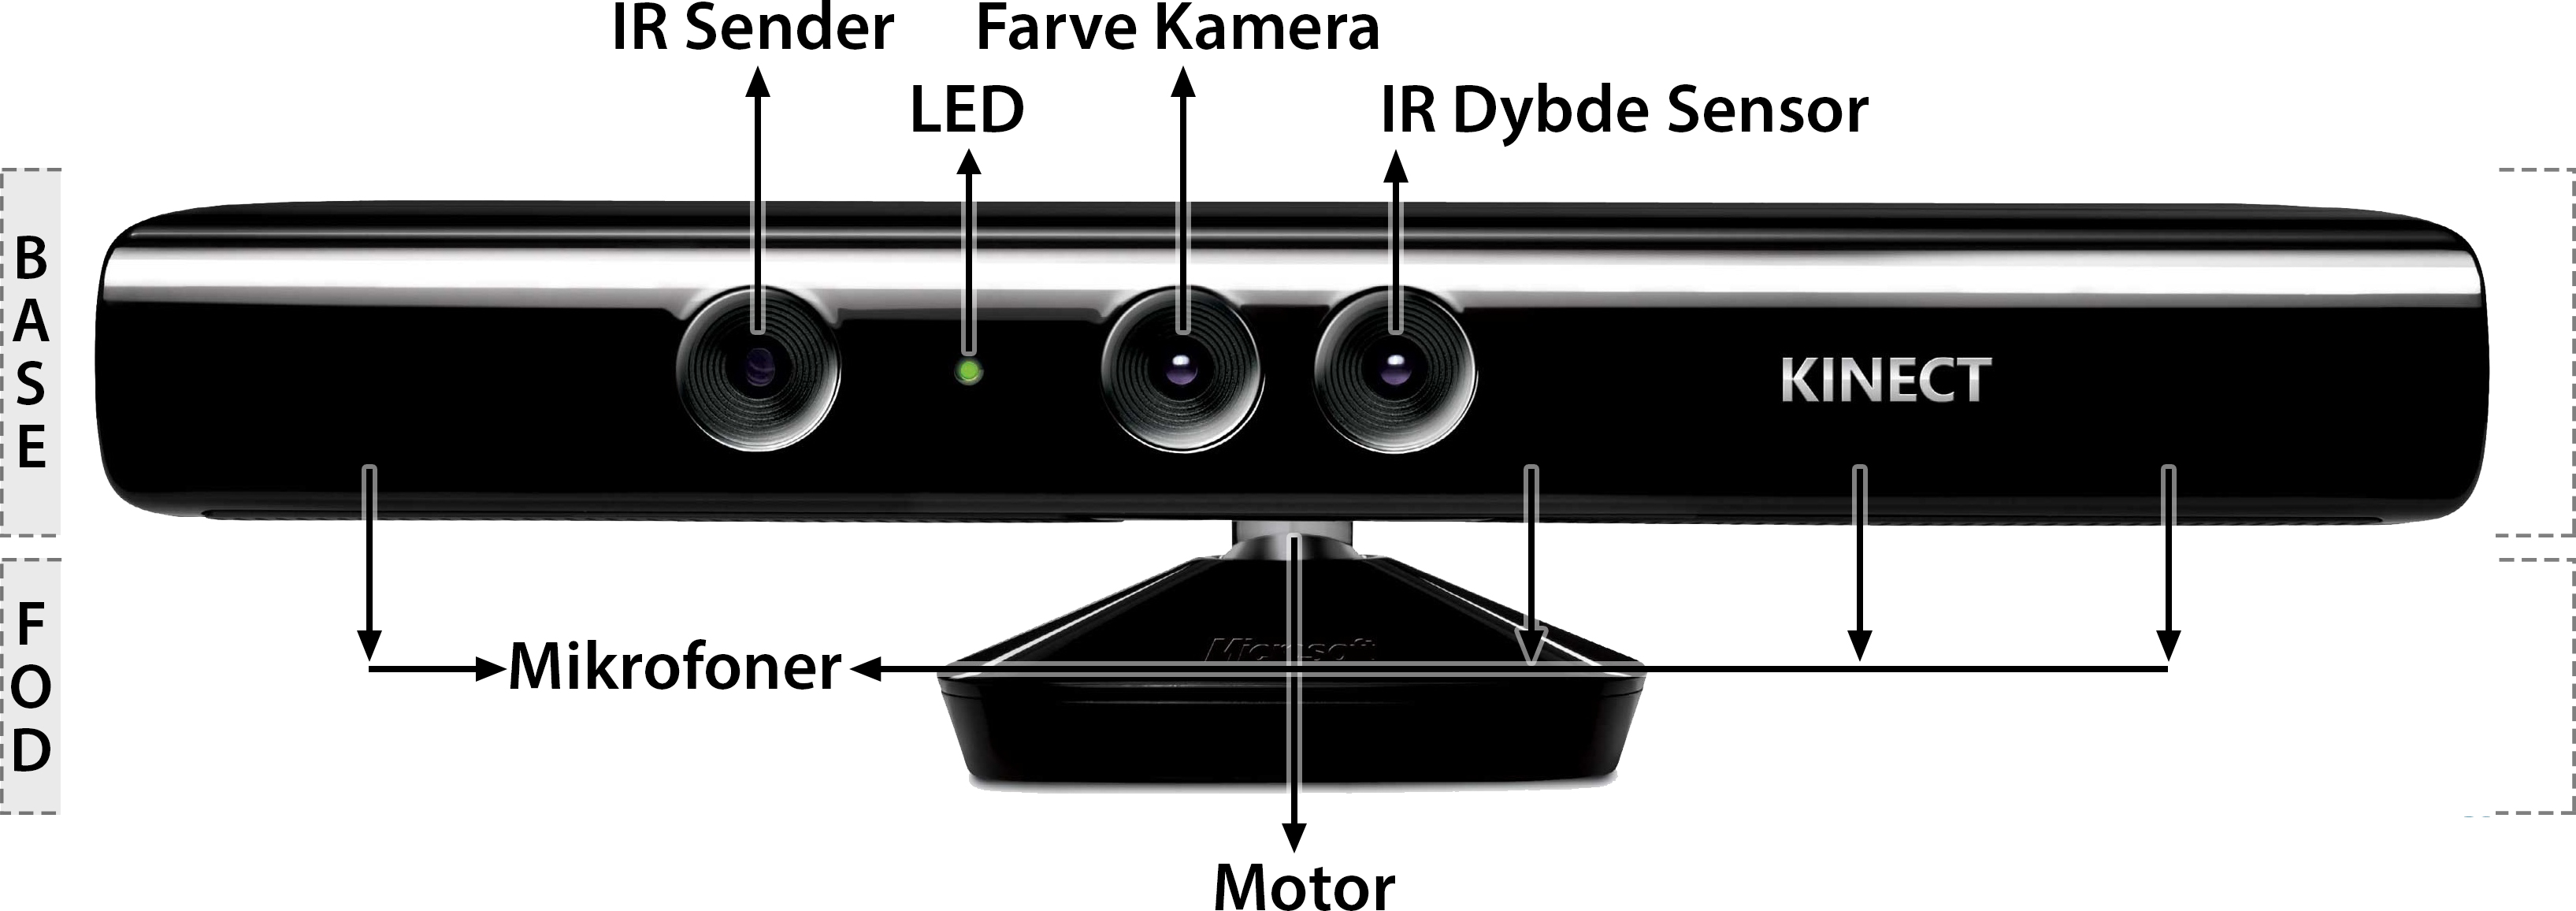
\includegraphics[width=1.0\textwidth]{kinect/kinect}
\caption{Illustration af occupancy grid for projekts kørselsmiljø for robotten.}
\label{map:occupancy_grid}
\end{figure}

\subsection{Occupancy Grid Mapping}


\section{Particle Filters}

\section{Sammenligning}

\